\chapter{0次ホールド}
    \providecommand{\FT}[1]{\mathcal{F}\parens*{#1}}
    \providecommand{\Ts}{T_\text{s}}
    \section{0次ホールドされた離散時間信号の周波数スペクトラム}
        \label{0次ホールドされた離散時間信号の周波数スペクトラム}
        \subsection{動機}
            離散時間信号を仮に量子化誤差なくDA変換できた場合の周波数スペクトラムを計算したい。
        \subsection{主張}
            $\xd:\integers\to\complexNumbers$ を離散時間信号とする。
            $\XDTFT$ を $\xd$ のDTFTとする。
            $\Ts>0$ をサンプル周期として $\xd$ の0次ホールドで生成した階段状の連続時間信号を $x$ とする。
            $u:\realNumbers\to\braces{0,1}$ を幅 $\Ts$ のパルスとする。
            \[
                u(t) = \begin{cases}
                    1 & 0\leq t < \Ts \\
                    0 & \text{otherwise}
                \end{cases}
            \]
            $x$ は次式で表される。
            \[ x(t) = \sum_{n=-\infty}^\infty \xd(n)u(t-n\Ts) \]
            次の図は $\Ts=1,\xd(n) = \sin\parens{2\pi n/12}\;(0\leq n\leq 24),\;\xd(n) = 0\;(n<0,24<n)$ の例である。
            \begin{figure}[H]
                \centering
                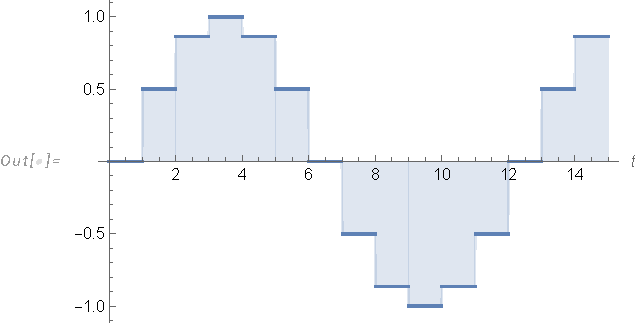
\includegraphics[keepaspectratio, scale=0.8]
                {\currfiledir/figs/x1.pdf}
                \caption{$x$の例}
                \label{figure:離散時間信号のDAC出力の例}
            \end{figure}
            以上の下, $x$ のFourier変換 $X$ は次式である。
            \[ X(\omega) = \frac{\Ts}{\sqrt{2\pi}}\exp\parens*{-i\frac{\Ts}{2}\omega}\parens*{\sinc \frac{\Ts}{2}\omega}\XDTFT(\omega) \]
            $\XDTFT(\omega)$ が $2\pi/\Ts$ 周期関数であることに注意すれば,$\XDTFT(\omega)$ の第1 Nyquist領域の形状が位相回転 $\exp\parens{-i \omega n\Ts}$ とレベル減衰 $\sinc\omega\Ts/2$ を伴いつつ周期的に無限に繰り返されていることがわかる。
            この現象は「アパーチャ効果」と呼ばれる。
            次の図は\ref{figure:離散時間信号のDAC出力の例}に対応する $X$ の例である。
            \begin{figure}[H]
                \centering
                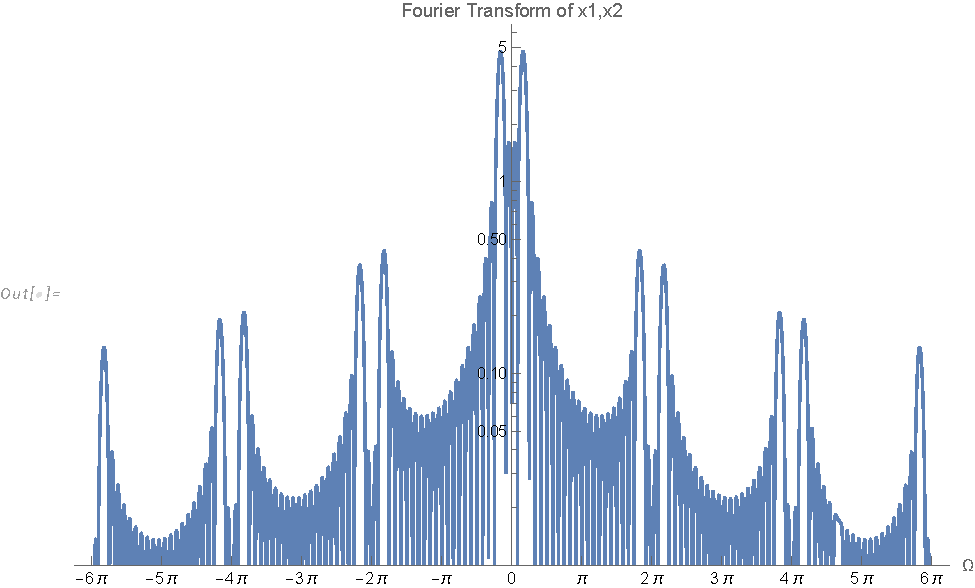
\includegraphics[keepaspectratio, scale=0.8]
                {\currfiledir/figs/FT_of_x1.pdf}
                \caption{$X$の例。横軸は正規化角周波数}
            \end{figure}
        \subsection{導出}
            \begin{proof}
                \quad\par
                \[ X(\omega) = \FT{\sum_{n=-\infty}^\infty \xd(n)u(t-n\Ts)}(\omega) = \sum_{n=-\infty}^\infty \xd(n)\FT{u(t-n\Ts)}(\omega) \tag{1} \]
                ここで次式が成り立つ。
                \begin{align*}
                    \FT{u(t-n\Ts)}(\omega) &= \exp\parens*{-i \omega n\Ts}\FT{u}(\omega) = \exp\parens*{-i \omega n\Ts}\frac{1}{\sqrt{2\pi}}\integrate{0}{\Ts}{\exp\parens*{-i\omega t}}{}{t} \\
                    &= \frac{i}{\omega\sqrt{2\pi}}\parens*{\exp\parens*{-i \omega\Ts}-1}\exp\parens*{-i \omega n\Ts} \\
                    &= \frac{i}{\omega\sqrt{2\pi}}\exp\parens{-i \omega n\Ts}\exp\parens{-i \omega\Ts/2}\parens*{\exp\parens*{-i \omega\Ts/2} - \exp\parens*{i \omega\Ts/2}} \\
                    &= \frac{i}{\omega\sqrt{2\pi}}\exp\parens{-i \omega n\Ts}\exp\parens{-i \omega\Ts/2}(-2i)\sin\frac{\omega\Ts}{2} \\
                    &= \frac{2}{\omega\sqrt{2\pi}}\exp\parens{-i \omega n\Ts}\exp\parens{-i \omega\Ts/2}\sin\frac{\omega\Ts}{2} \\
                    &= \frac{\Ts}{\sqrt{2\pi}}\exp\parens{-i \omega n\Ts}\exp\parens{-i \omega\Ts/2}\sinc\frac{\omega\Ts}{2}
                \end{align*}
                これを式(1)に適用して次式を得る。
                \begin{align*}
                    X(\omega) &= \sum_{n=-\infty}^\infty \xd(n)\frac{\Ts}{\sqrt{2\pi}}\exp\parens{-i \omega n\Ts}\exp\parens{-i \omega\Ts/2}\sinc\frac{\omega\Ts}{2} \\
                    &= \frac{\Ts}{\sqrt{2\pi}}\exp\parens{-i \omega\Ts/2}\sinc\frac{\omega\Ts}{2} \sum_{n=-\infty}^\infty \xd(n)\exp\parens{-i \omega n\Ts} \\
                    &= \frac{\Ts}{\sqrt{2\pi}}\exp\parens*{-i\frac{\Ts}{2}\omega}\parens*{\sinc \frac{\Ts}{2}\omega}\XDTFT(\omega)
                \end{align*}
            \end{proof}
    \section{inverse-sinc-filter}
        \subsection{背景}
            離散時間信号をDA変換した結果のFourier変換には次式で表される変化が積の形で含まれることを\ref{0次ホールドされた離散時間信号の周波数スペクトラム}で述べた。
            \[ \sinc \frac{\Ts}{2}\omega = \sinc \frac{\Omega}{2} \]
            ここに $\Ts$ はサンプリング周期, $\Omega$ は正規化角周波数である。
            変化の中には上式の他に $\exp\parens*{-i\frac{\Ts}{2}\omega}$ という項も含まれるが,これは一定の群遅延が加わる(線形位相特性)だけであり,実用上無害なので無視する。
            次の図は $\abs{\sinc \frac{\Omega}{2}}$ をプロットしたものである。
            \begin{figure}[H]
                \centering
                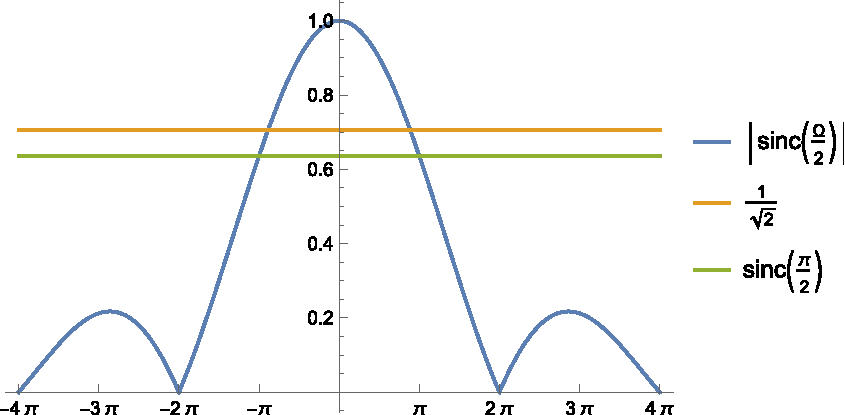
\includegraphics[keepaspectratio, scale=0.6]
                {\currfiledir/figs/sinc-shaped_gain_distortion_with_ideal_DA.pdf}
                \caption{量子化誤差のないDA変換結果の sinc 状ゲイン歪み}
            \end{figure}
            上の図から,第1 Nyquist 領域の端 $-\pi, \pi$ で約 -3dB のゲイン低下が生じていることが解る。
            実は0次ホールドで出力する直前に,上手く設計された10タップ程度の feedforward フィルタを掛けてこの影響を緩和し,下図のようなゲイン特性に変更できる。
            このフィルタは「inverse-sinc フィルタ」と呼ばれる。
            \begin{figure}[H]
                \centering
                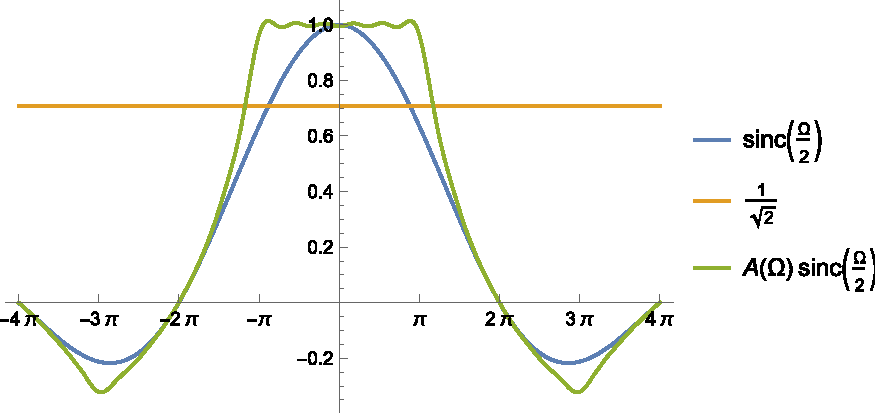
\includegraphics[keepaspectratio, scale=0.6]
                {\currfiledir/figs/mitigated_distortion_with_inverse-sinc_filter.pdf}
                \caption{inverse-sinc フィルタによって緩和されたゲイン歪み(凡例の3つ目の曲線)}
                \label{inverse-sinc フィルタによって緩和されたゲイン歪み}
            \end{figure}
            inverse-sinc フィルタは $[-\pi, \pi]$ で sinc 状歪みの逆特性を近似するフィルタである。
            DA変換の対象とする信号は通常,標本化定理を念頭に置いてスペクトラムが $[-\pi,\pi]$ の領域に収まる信号であるから,上述の補正が十分に機能する。
            以下ではこのフィルタの設計方法の1つを述べる。
        \subsection{係数の導出}
            大雑把に言えば,フィルタ係数に対応する DTFT が $[-\pi,\pi]$ で $1/\sinc(\Omega/2)$ を近似するように最小二乗法で係数を決定する。
            \par
            フィルタ係数 $a:\integers\to\realNumbers$ は偶対称な実数値関数とし,非零の係数の個数を奇数とする。
            数式で述べれば $N\in\naturalNumbers,\;\forall n\in\integers\;a(-n) = a(n),\forall n>N\;a(n) = 0$ である。
            この制約条件が唯一の方法ではないだろうが,後に見るようにこれで十分な性能を得られる。
            \par
            $a$ の DTFT を $A$ とする。すなわち
            \[ A(\Omega) = \sum_{n=-N}^N a(n)\exp(-i\Omega n) = a(0) + 2\sum_{n=1}^N a(n)\cos(\Omega n) = \bm{v}(\Omega)^\top\bm{a} \]
            ここに $\bm{v}(\Omega) \coloneq [1, 2\cos\Omega,\dots,2\cos N\Omega]^\top\in\realNumbers^{N+1},\;\bm{a} = [a(0),\dots,a(N)]^\top\in\realNumbers^{N+1}$ である。
            $[-\pi,\pi]$ で $A$ が $1/\sinc(\Omega/2)$ を近似するように次式を最小化する $a$ を求める。
            \[ \integrate{-\pi}{\pi}{\norm{A(\Omega) - 1/\sinc(\Omega/2)}_2^2}{}{\Omega} \tag{1} \]
            被積分関数の中身を展開すると次式を得る。
            \[ \norm{A(\Omega) - 1/\sinc(\Omega/2)}_2^2 = \bm{a}^\top\bm{v}(\Omega)\bm{v}(\Omega)^\top\bm{a} - \frac{2}{\sinc(\Omega/2)}\bm{v}(\Omega)^\top\bm{a} + 1/\sinc(\Omega/2)^2 \]
            これを式(1)に適用すると次式を得る。
            \[ (1) = \bm{a}^\top M\bm{a} - 2\bm{m}^\top\bm{a} + \integrate{-\pi}{\pi}{1/\sinc(\Omega/2)^2}{}{\Omega} \tag{2} \]
            ここに $M,\bm{m}$ は次式で定義される数である。
            \[ M \coloneq \integrate{-\pi}{\pi}{\bm{v}(\Omega)\bm{v}(\Omega)^\top}{}{\Omega} = 2\pi\diag{1,2,2,\dots,2},\quad \bm{m} = \integrate{-\pi}{\pi}{\bm{v}(\Omega)^\top/\sinc(\Omega/2)}{}{\Omega} \]
            $\bm{m}$ は数値計算で求める。
            式(2)の中で $\bm{a}$ に依存しない項を無視すると,最小化すべき関数は次式である。
            \[ f_\text{cost}(\bm{a}) = \bm{a}^\top M\bm{a} - 2\bm{m}^\top\bm{a} \]
            これは狭義凸関数であり $(\nabla f_\text{cost})(\bm{a}) = 2(M\bm{a} - \bm{m})$ なので $f$ を最小化する $\bm{a}$ を $\bm{a}_\text{opt}$ とするとこれは $M^{-1}\bm{m} = \diag{m_0,m_1 /2,\dots,m_N /2}/(2\pi)$ である。
            ここに $m_i\;(i=0,1,\dots,N)$ は $\bm{m}$ の第 $i$ 要素である。
        \subsection{数値例}
            $N=5$ のとき $\bm{a}_\text{opt} \approx [1.166240, -0.106996, 0.034475, -0.016454, 0.009530, -0.006189]^\top$ を得る。
            次の図はこの係数をプロットしたものである。
            \begin{figure}[H]
                \centering
                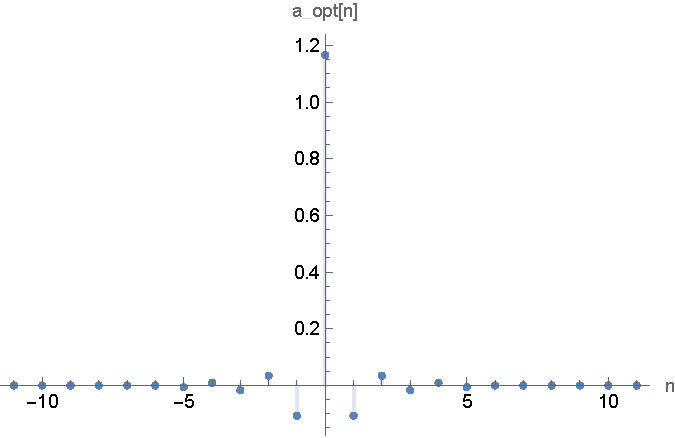
\includegraphics[keepaspectratio, scale=0.6]
                {\currfiledir/figs/coeffs_of_inverse-sinc_filter.pdf}
                \caption{inverse-sinc フィルタの係数($N$=5)}
            \end{figure}
            次の図は,この係数に対応するフィルタのインパルス応答の DTFT と $1/\sinc(\Omega/2)$ を比較したものである。
            \begin{figure}[H]
                \centering
                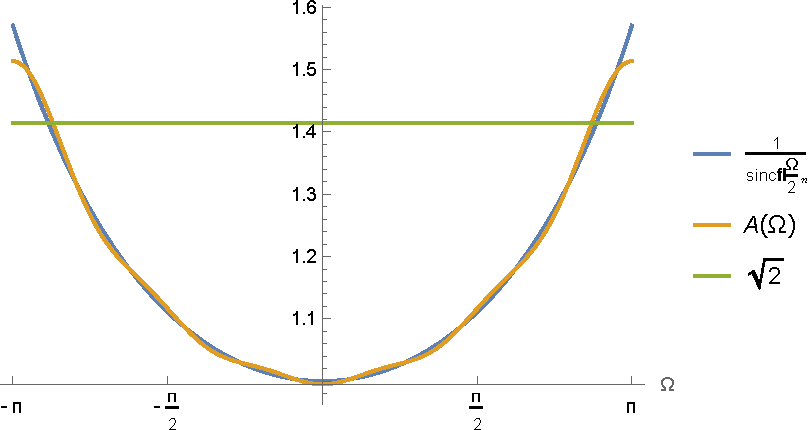
\includegraphics[keepaspectratio, scale=0.6]
                {\currfiledir/figs/inverse-sinc_approximation.pdf}
                \caption{inverse-sinc フィルタのインパルス応答の DTFT}
            \end{figure}
            このフィルタを使ってゲイン歪みを緩和したのが先に挙げた図\ref{inverse-sinc フィルタによって緩和されたゲイン歪み}である。
